\chapter{Management Summary}
	\captionsetup[figure]{labelformat=empty} % disable figure numbering

	
	\section{Ausgangslage}
	
	"'Entwurfsentscheidungen als Projektplanungsinstrument"', kurz \eeppi\. 
	Diesem Thema widmet sich die vorliegende Arbeit und befasst sich mit der Frage, 
	ob sich aus Projektentscheidungen Aufgaben ableiten lassen. 
	Weiterhin wird untersucht, ob sich dieser Prozess automatisieren lässt. 

	Jedes Projekt erfordert das Treffen von Entscheidungen, 
	wobei aus einer bestimmten Entscheidung häufig ähnliche Aufgaben resultieren. 
	Sowohl auf Seite der Entscheidungsverwaltung wie auf Seiten der Projektplanung existieren bereits verschiedene Werkzeuge. 
	Ziel von \eeppi\ ist es, eine Brücke zwischen Entscheidungsmanagement und Projektplanung zu bauen.
	
	\begin{figure}[H]
		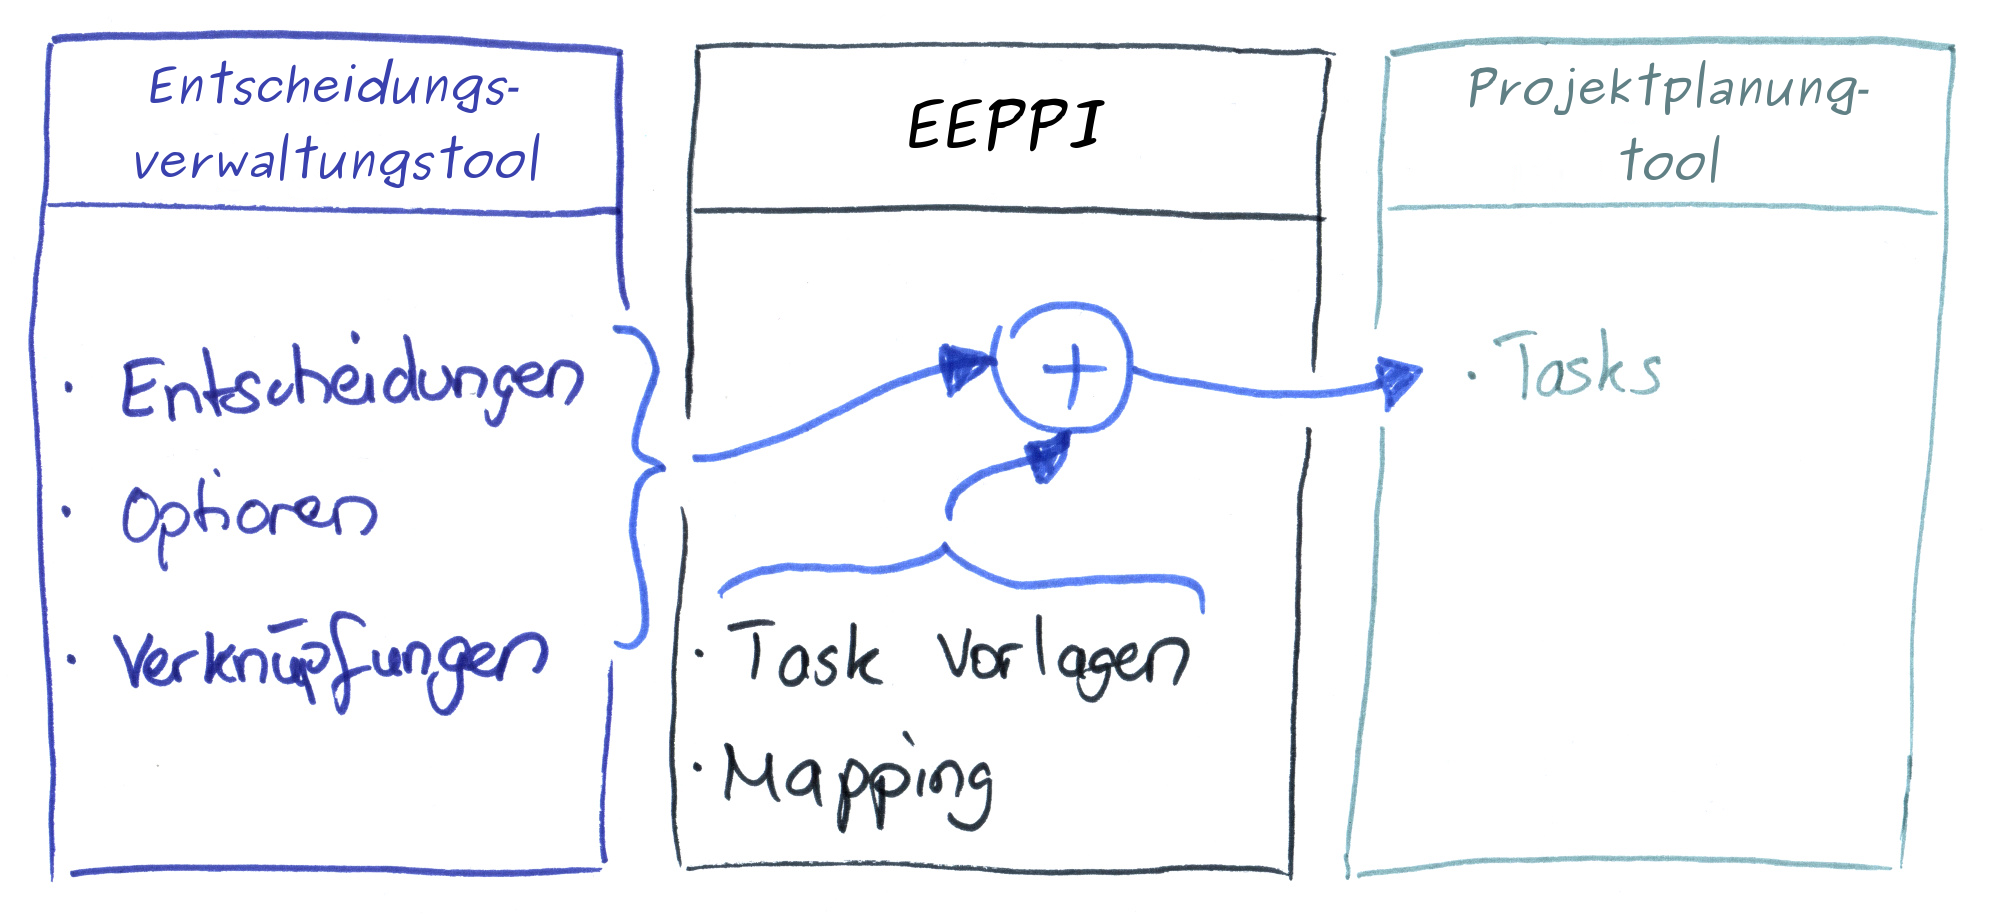
\includegraphics[width=0.8\textwidth]{introduction/img/eeppiVision.png}
		\centering
		\caption{EEPPI bildet eine Brücke zwischen Entscheidungsmanagement- und Projektplanung}
		\label{fig:eeppiBridgeBetweenDecisionsAndTasks}
	\end{figure}
	
	
	\section{Vorgehen}
	
	Aufbauend auf den Schnittstellen von Wissensverwaltungssystemen und Projektplanungstools wurden eine Applikation und eine Oberfläche entworfen, 
	die eine flexible Konfiguration der Schnittstellen ermöglichen. 
	Benutzer sollen Aufgabenvorlagen erstellen, diese mit Entscheidungen verknüpfen und in ein Projektplanungstool übertragen können. 

	Mittels Prototyp wurde die Machbarkeit dieses Ansatzes überprüft 
	und anschliessend im Rahmen mehrerer Iterationen eine Webapplikation entwickelt. 
	Zusammen mit dem Betreuer als Ansprechpartner der Kundengruppe wurden Usability- und Workflowtests durchgeführt, 
	um Benutzeroberfläche und Datenfluss vom Entscheidungsverwaltungssystem bis ins Projektplanungstool zu validieren. 
	Abschliessend folgte zur Stabilisierung eine Überarbeitungsphase.
	
	
	\section{Ergebnis}
		
	Im Rahmen der Arbeit wurde eine Webapplikation entwickelt, 
	die mögliche Entscheidungen aus einem angebundenen Wissensverwaltungssystem bezieht 
	und dem Benutzer mit einem Metamapping ermöglicht,
	Projektentscheidungen mit eigenen Aufgaben zu verknüpfen. 
	
	\begin{figure}[H]
		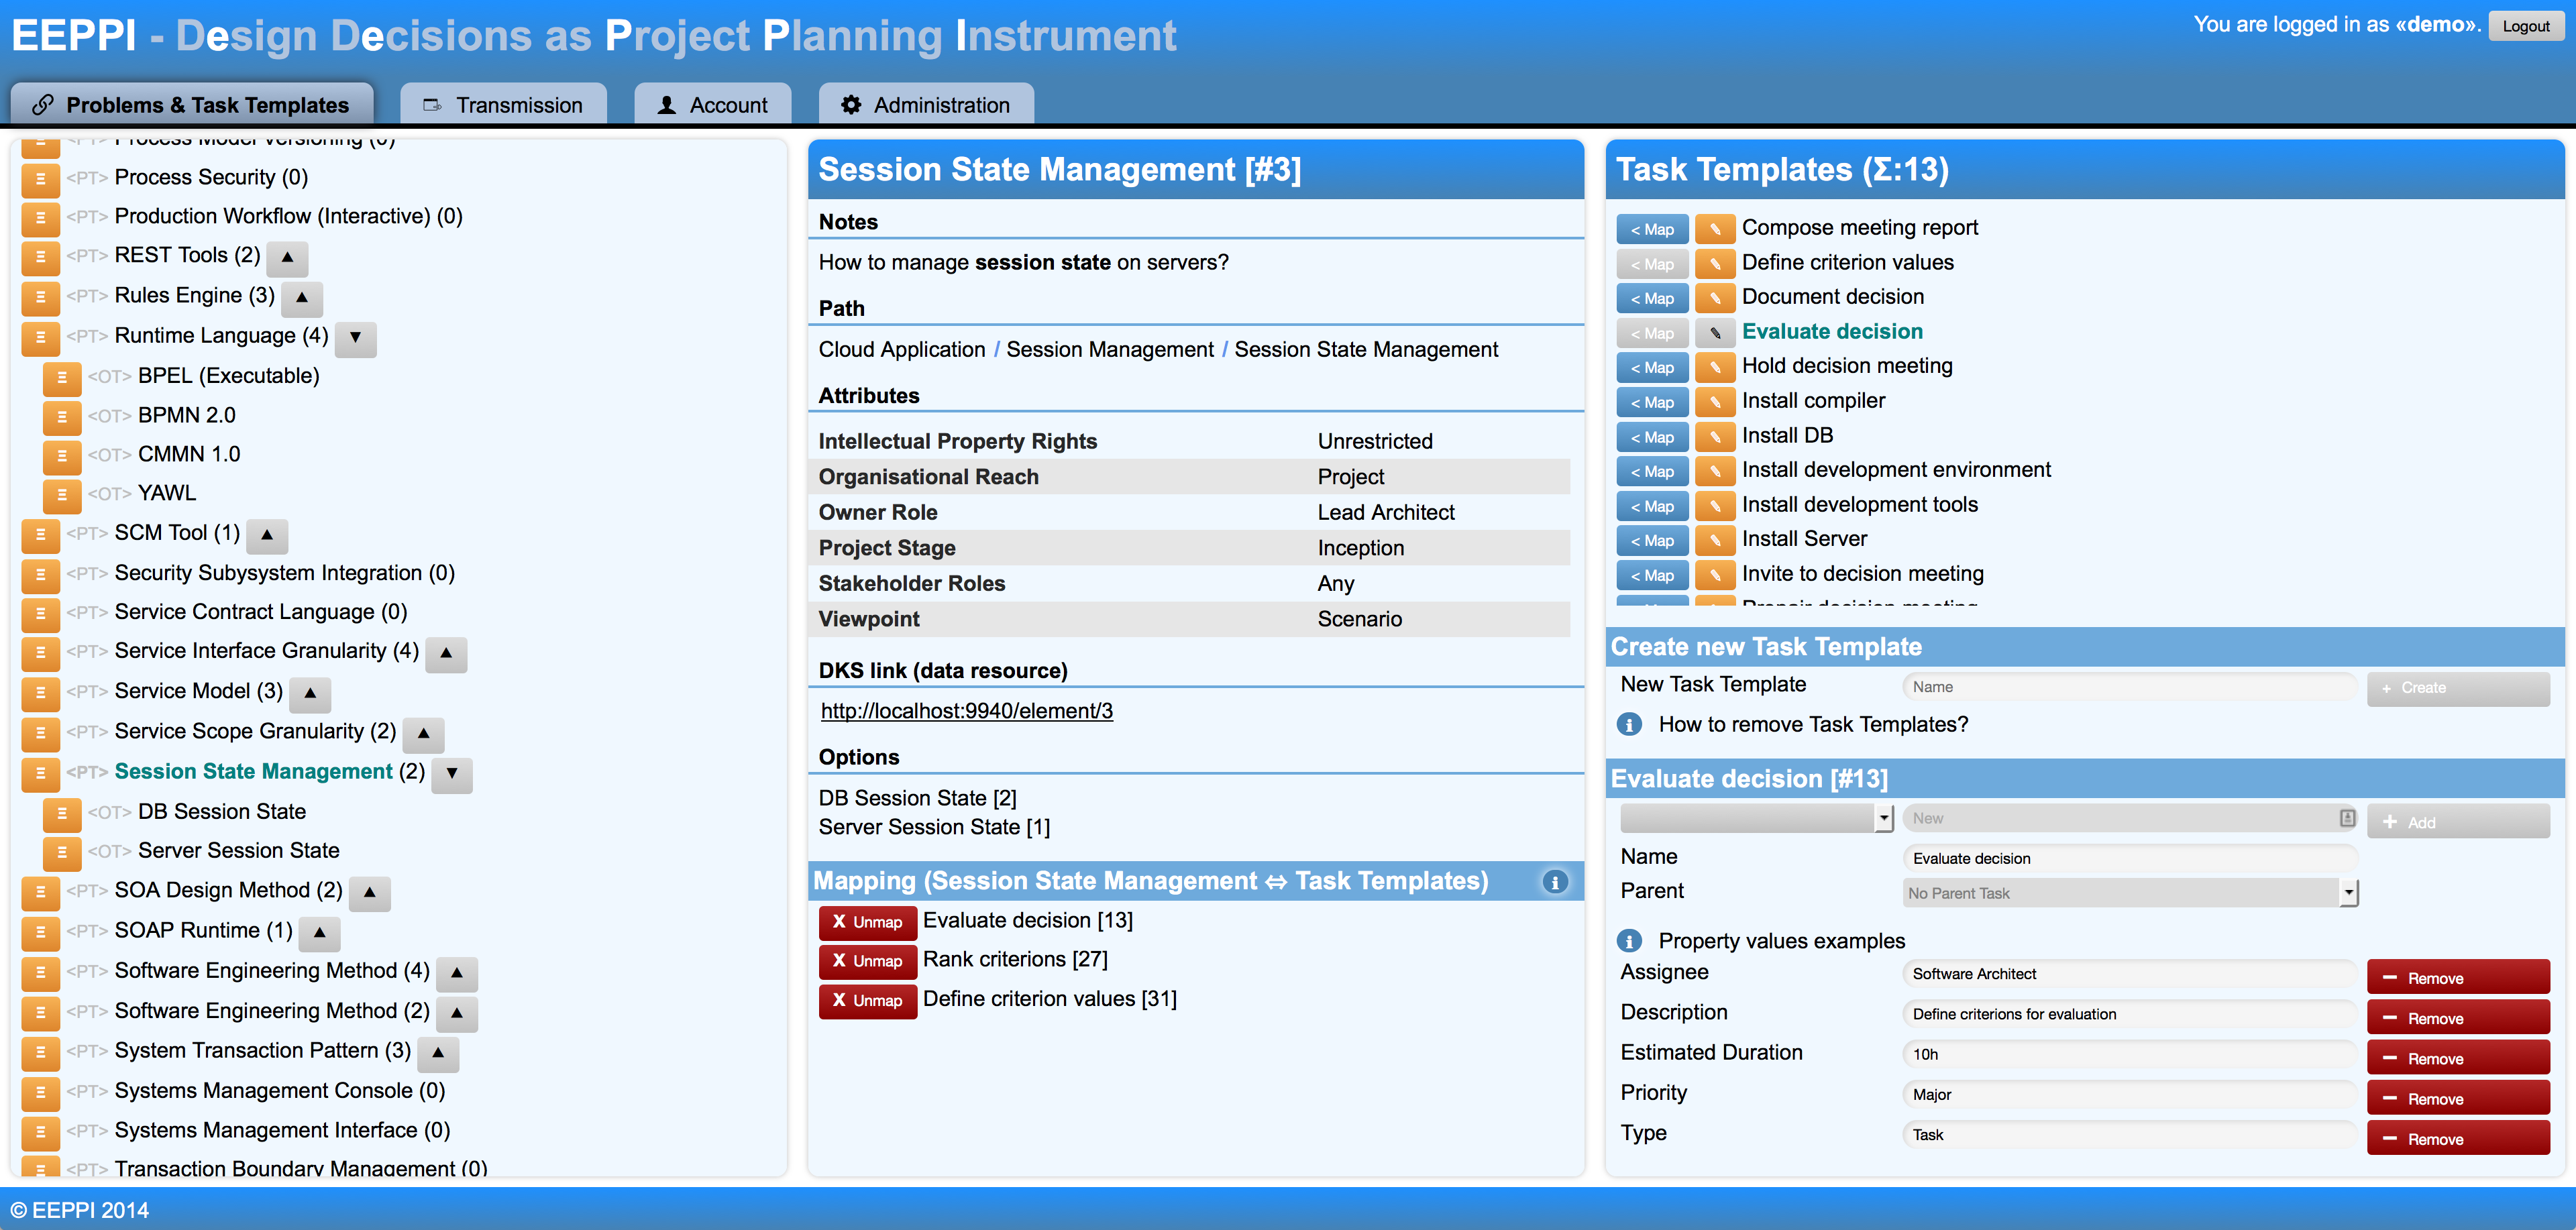
\includegraphics[width=\textwidth]{introduction/img/eeppiDecisionsAndTaskTemplates.png}
		\centering
		\caption{Metamapping in EEPPI: Verknüpfen von Entscheidungen und Aufgabenvorlagen}
		\label{fig:metamapping}
	\end{figure}	
	
	Über einen Administrationsbereich konfiguriert der Benutzer die Applikation nach seinen Bedürfnissen. 
	Beispielsweise kann der Benutzer selbst den Aufbau der zu generierenden Aufgaben steuern. 
	Ein dazu entwickelter Templatingmechanismus ermöglicht ihm, eigene Verarbeitungsfunktionen, sogenannten Prozessoren, zu verwenden. 
	
	\begin{figure}[H]
		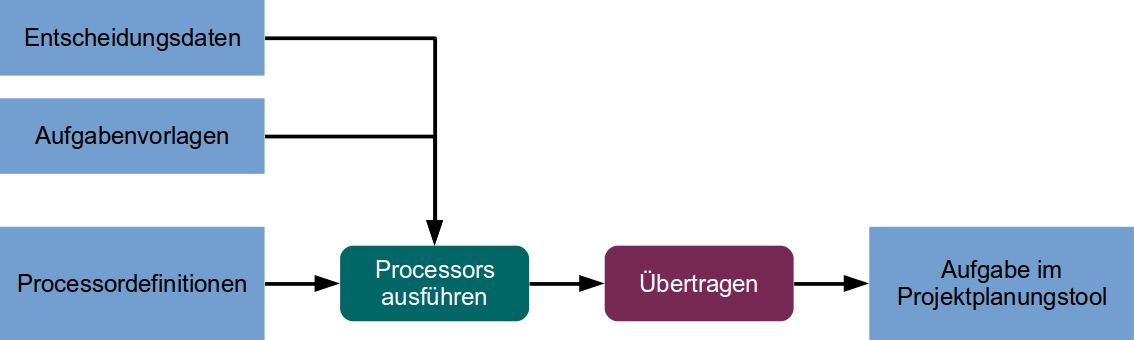
\includegraphics[width=\textwidth]{introduction/img/simpleProcessWorkflow.jpg}
		\centering
		\caption{Übertragung: Ausführen von Prozessoren und Übermitteln der Aufgaben an ein Projektplanungstool}
		\label{fig:metamapping}
	\end{figure}
	
	\eeppi\ zeigt, was kommerzielle Produkte in diesem Bereich anbieten könnten, 
	aber auch die Design-Herausforderungen einer solchen Software: 
	Hohe Flexibilität und Konfigurierbarkeit. 
	Mit EEPPI ist dies bereits gelungen; es gibt jedoch noch viele Erweiterungsmöglichkeiten. 
	\eeppi\ legt somit einen wichtigen Meilenstein im Forschungsbereich des interdisziplinären Entscheidungs- und Projektmanagements 
	und zeigt einen möglichen Entwicklungspfad für zukünftige Tools auf.
	
	\captionsetup[figure]{labelformat=default} % reenable figure numbering